\documentclass[twocolumn]{article}
\usepackage[utf8]{inputenc}
\usepackage{abstract}
\usepackage{graphicx}
\usepackage{amsmath, amssymb}
\usepackage{hyperref}
\usepackage{cite}
\usepackage{caption}
\usepackage{subcaption}
\usepackage{geometry}
\usepackage{booktabs}
\usepackage{float}
\geometry{margin=1in}

\title{Predicting Turtle Age with Various Machine Learning Models}
\author{
 Elias Schlie \\
 u783766 \\
 Tilburg University \\
  \texttt{e.p.schlie@tilburguniversity.edu}
}
\date{}

\begin{document}


\twocolumn[
  \maketitle

  \begin{abstract}
 With the aim of supporting wildlife conservation agencies (WCAs) in their mission to protect turtles, this report presents different machine learning algorithms to predict turtle age from their features. The algorithms used include linear regression, polynomial regression, and a K nearest-neighbor (KNN) algorithm. After a thorough comparison, the second-degree polynomial regressor emerged as the best-performing algorithm, with predictions differing only 1.5 years from the target variable on average. 
  \end{abstract}
  \vspace{3em}
]

\section{Introduction}

In their pursuit of protecting turtles, many WCAs are following a practice that causes risk to the turtles they are trying to protect. 
This practice involves determining the age of a turtle by slicing their shell and counting the number of growth rings inside. 
Knowing the age of turtles is an important data point for WCAs as it helps them determine where to direct their efforts. 
Unfortunately, this practice is not only time-consuming but also dangerous for the turtles. 
Naturally, it follows, that a way to accurately determine turtle age from non-invasive data would provide a lot of value towards their protection. 
The following report compares, multiple machine learning models for the purpose of predicting the number of growth rings a turtle has from a set of features that can be measured non invasively.

\section{Data and Preprocessing}
% Describe the dataset, relevant features, and how you prepared/split the data.

\subsection{Dataset Description}
The turtle-2.csv dataset contains information on 4,177 turtles, including their sex, length, diameter, height, and number of rings. 
It also provides detailed weight measurements, divided into whole weight, shucked weight, shell weight, and visceral weight.

\subsection{Outlier Detection and Removal}

Upon closer investigation of the data, it stands out that four turtles have implausible height values. 
Two of them have heights of 0 cm, while the other two have heights of 51.5 cm and 113 cm, which is far outside the height distribution in the rest of the dataset. 
As apparent in Figure~\ref{fig:height_rings_pre_clean}, other turtles maximally reach a height of 25 cm.
\begin{figure}[h]
    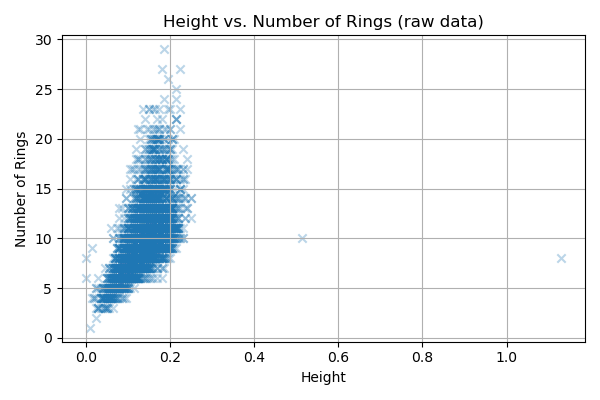
\includegraphics[width=\linewidth]{Figures/Height_vs._Number_of_Rings__raw_data_.png}
    \caption{Scatterplot showing the relationship between turtle height and number of rings before outlier removal.}
    \label{fig:height_rings_pre_clean}
\end{figure}
Those four measurements are highly biologically implausible and were therefore removed from the dataset, leaving 4173 turtles. Figure~\ref{fig:height_rings_post_clean} shows the more balanced relationship between turtle height and number of rings resulting from removing the outliers.

\begin{figure}[h]
    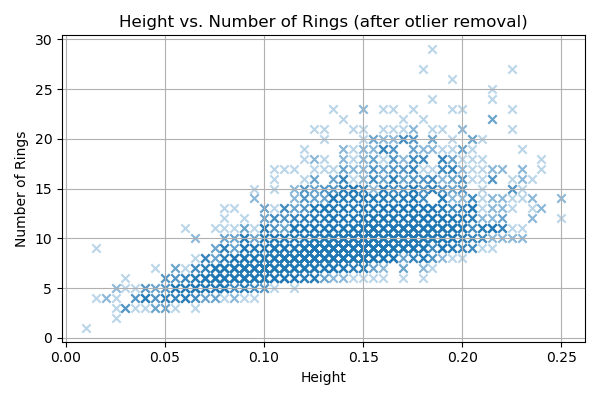
\includegraphics[width=\linewidth]{Figures/Height_vs._Number_of_Rings__after_otlier_removal_.png}
    \caption{Scatterplot showing the relationship between turtle height and number of rings after outliers have been removed.}
    \label{fig:height_rings_post_clean}
\end{figure}

\subsection{Statistics of numerical features}

With the exception of sex, all features in the turtle-2.csv dataset are numerical. Notably, all features fall into roughly the same range with means between 0.250 and 2.825. Only the target variable, number of rings, has a mean of 9.936, not matching the feature variables. Table~\ref{tab:desc_stats} lists the mean, standard deviation (std), minimum (min), and maximum (max) of all numerical features in the dataset.
\begin{table}[t]
    \caption{Descriptive Statistics}
    \label{tab:desc_stats}
    \begin{tabular}{lrrrr}
    \toprule
     & mean & std & min & max \\
    \midrule
 Length & 0.524 & 0.120 & 0.075 & 0.815 \\
 Diameter & 0.408 & 0.099 & 0.055 & 0.650 \\
 Height & 0.139 & 0.038 & 0.010 & 0.250 \\
 Whole weight & 0.829 & 0.490 & 0.002 & 2.825 \\
 Shucked weight & 0.359 & 0.222 & 0.001 & 1.488 \\
 Viscera weight & 0.181 & 0.110 & 0.001 & 0.760 \\
 Shell weight & 0.239 & 0.139 & 0.002 & 1.005 \\
 Rings & 9.936 & 3.225 & 1.000 & 29.000 \\
    \bottomrule
    \end{tabular}
\end{table}
To further visualize the data, scatterplots of the relationship between each individual feature with the number of rings can be found in figure~\ref{fig:all_features_datasets} in the appendix.

A heatmap of the correlations between the numeric features reveals that all of them are strongly correlated with the exception of the number of rings which shows weaker correlations with other features than they do internally (see Figure~\ref{fig:heatmap}). 
Correlations between different features range from 0.837 between height and shucked weight to 0.987 between diameter and length. 
In contrast, number of rings only reaches correlations between 0.421 and 0.628 which is markedly less. Rings correlates most strongly with shell weight and height.

\subsection{Analysis of the Categorical Feature: Sex}

The only categorical feature in the dataset is sex, which takes on the three values M, F, and I. The boxplots of figure~\ref{fig:gender_boxplots} show the distributions of number of rings for turtles grouped by gender, revealing that turtles with the sex I seem to be younger on average. Statistical analysis shows that sex is significantly correlation with ring number. A one-way ANOVA reveals F = 499.33 with p \textless{} .001 and post-hock T-tests show that all means differ significantly (p \textless{} .001), but the effect is most pronounced between I and the other two genders. The effect size of differences follows the same pattern with Cohen's d \textgreater{} 1 between I and M, and I and F (For the exact values, see table~\ref{tab:gender_comparisons} in the Appendix). To make the sex feature usable for machine learning, it was one hot encoded into the three features Sex\_F, Sex\_M, and Sex\_I. 

\subsection{Data Splitting Strategy}
The dataset was split into three buckets. 80\% was allocated for training, 10\% for validating, and 10\% for testing the models. 
To ensure that the distribution of rings stays preserved in each set, the data was stratified into 5 bins before splitting, ensuring equal proportions of each bin in each set. For the binning process, the \texttt{KBinsDiscretizer} from the \texttt{scikit-learn} python library was used with the quantile strategy. The created bin indices were used with the \texttt{train\_test\_split} function from \texttt{scikit-learn} to produce the desired sets. A test was conducted after binning to confirm that the bins were equally distributed across sets. Reproducibility was ensured by setting \texttt{random\_state=1} for the split function and using \texttt{scikit-learn} version 1.6.1 throughout the whole report. Due to the fact that all values are already in ranges close to 1, the features were not normalized.


\section{Model Training and Tuning}
% Discuss the different regressors (Linear, Polynomial, KNN), how you tuned hyperparameters, and how you decided on the best model.

%\subsection{Baseline}
%The \texttt{DummyRegressor} from \texttt{scikit-learn} was used to determine a baseline for evaluating model performance.
%The strategy for this regressor was to always predict the mean of the dataset, independently of the input.

\subsection{Linear Regression}
The first machine learning model used to predict the number of rings of a turtle was the \texttt{LinearRegression} model from \texttt{scikit-learn}. This model doesn't require any hyperparameter tuning and was therefore used as is in the later model comparison.

\subsection{Polynomial Regression}

Using the \texttt{PolynomialFeatures} class from the \texttt{scikit-learn} library, features were transformed into polynomial features of degrees 2 to 5. 
\texttt{LinearRegression} models, like the one mentioned in the previous section, were then trained on the expanded sets of features and compared on the basis of their mean squared error (MSE) on the validation data.
The polynomial regressor with degree 2 performed best out of all, displaying the lowest MSE. For the higher degree polynomials, overfitting was clearly visible, as their performance on the training set increased while their MSE on the validation set got markably worse.

\subsection{K-nearenst neighbor model}

The final model type in this comparison is the KNN algorithm implemented through the \texttt{KNeighborsRegressor} class form \texttt{scikit-learn}.
KNNs with hyperparameter k = \{1, 3, 6, 10\} were compared on the validation set with the model using k=6 achieving the lowest mean squared error.

\subsection{Performance Comparison and Model Selection}

To choose the best overall model, the test set MSEs of the linear regressor, the 2nd-degree polynomial regressor, and the KNN with k=6 were compared. The polynomial of degree two achieved the lowest MSE and was therefore chosen as the best model. Table~\ref{tab:model_comparisons} includes detailed performance metrics including MSE, mean average error (MAE), and R2 score for all models. Figure~\ref{fig:model_predictions} further visualizes their predictions against the true ring values in scatterplots.

\section{Results and Discussion}
% Present performance metrics (R2, MSE, MAE) on the test set, summarize cross-validation and provide error analyses. Highlight model strengths and weaknesses.

The following section dives into the performance of the 2nd-degree polynomial, from this point on referred to as "the model".

\subsection{Cross validation performance}

To get a more reliable estimate of the performance of the model, a 10-fold-cross-validation was performed, collecting its MSE, MAE, and R2 score over different parts of the dataset (see figure~\ref{fig:polynomial_fold_valuation} for performance on each fold).
The model reached an average MSE of 4.452, an average MAE of 1.493, and an average R2 score of 0.569, indicating that the model can explain around 56.9\% of the variance of rings in the dataset.

\subsection{Feature importance}

Because the model is polynomial, the 10 initial features were expanded into 65 different features, all being weighted by their individual coefficient. By looking at the coefficients produced by the fold with the lowest MSE it stands out that the 15 features with the greatest coefficients are all polynomial. The three most influential features are diameter times height, diameter squared, and height times shucked weight. The features with the lowest weight are all related to gender, with all combinations of one gender times another being multiplied by zero. Figure~\ref{fig:coefficient_magnitudes} visualizes the magnitudes of coefficients in a sorted bar graph. The intercept of the model resides at -0.79.

\subsection{Error analysis}
The model performed worst on fold number 5 where it achieved an MSE of 5.823, an MAE of 1.637, and an R2 error of 0.517. The errors of this specific fold were analyzed in more detail to find potential biases or weaknesses in the model. Figure~\ref{fig:over_underprediction_density} compares kernel density estimates of the distributions of over and under-predicted instances with the distribution in all samples. It stands out that, while length, diameter, and height all show similar distributions, over-prediction becomes slightly more prevalent as other features increase.
Plotting the error magnitude per feature reveals that it is positively correlated with feature value in all values. Only for sucked weight and visceral weight the p-value for this correlation says above 0.01. Scatterplots of this interaction can be found in figure~\ref{fig:error_magnitude_by_feature} which also includes lines of best fit with their r and p values for each interaction.


\section{Conclusion}
% Conclude with your main findings and possible future improvements.

To conclude, the second-degree polynomial was found to be the best model for predicting the number of rings of turtles in the turtles-2.csv dataset. The predictions of this model are off by approximately 1.5 years on average without extreme outliers as indicated by a relatively low MSE. In total, this regressor can explain 56.9\% of the variance in the number of rings of the sample. Those metrics, while maybe not enough for rigorous studies, indicate that this model can be a valuable help for WCAs to estimate turtles' age without having to engage in the time-consuming and potentially dangerous invasive measurement. More data and better non-invasive measurements are needed to further improve the quality of predictions.


\bibliographystyle{plain}
\bibliography{references}

\onecolumn
\appendix
\newpage

\section{Tables}
\renewcommand{\thetable}{A.\arabic{table}}
\setcounter{table}{0}

\begin{table}[H]
    \centering
    \caption{Sorted correlations between rings and other features}
    \label{tab:correlations}
    \begin{tabular}{lr}
    \toprule
     & Rings \\
    \midrule
 Shell weight & 0.628 \\
 Height & 0.610 \\
 Diameter & 0.575 \\
 Length & 0.557 \\
 Whole weight & 0.541 \\
 Viscera weight & 0.504 \\
 Shucked weight & 0.421 \\
    \bottomrule
    \end{tabular}
\end{table}
    

\vfill

\begin{table}[H]
    \centering
    \caption{Statistical comparisons of number of rings between genders}
    \label{tab:gender_comparisons}
    \begin{tabular}{llll}
        \toprule
        & M vs F & M vs I & F vs I \\
        \midrule
 t-statistic & -3.681 & 27.188 & 29.465 \\
 p-value & \textless{}0.001 & \textless{}0.001 & \textless{}0.001 \\
 Cohen's d & -0.139 & 1.016 & 1.154 \\
        \bottomrule
    \end{tabular}
\end{table}

\vfill

% Work on this!
\begin{table}[H]
    \center
    \caption{Final models}
    \label{tab:model_comparisons}
    \begin{tabular}{lllrrr}
    \toprule
 Molel & Hyperparameters & MSE & MAE & R2 \\
    \midrule
 Linear Regression & NaN & 5.269 & 1.633 & 0.507 \\
 Polynomial Regression & degree=5 & 4.659 & 1.508 & 0.564 \\
 KNN & k=6 & 4.881 & 1.506 & 0.543 \\
    \bottomrule
    \end{tabular}
\end{table}

\newpage
\section{Figures}
\renewcommand{\thefigure}{A.\arabic{figure}}
\setcounter{figure}{0}

\begin{figure}[H]
    \center
    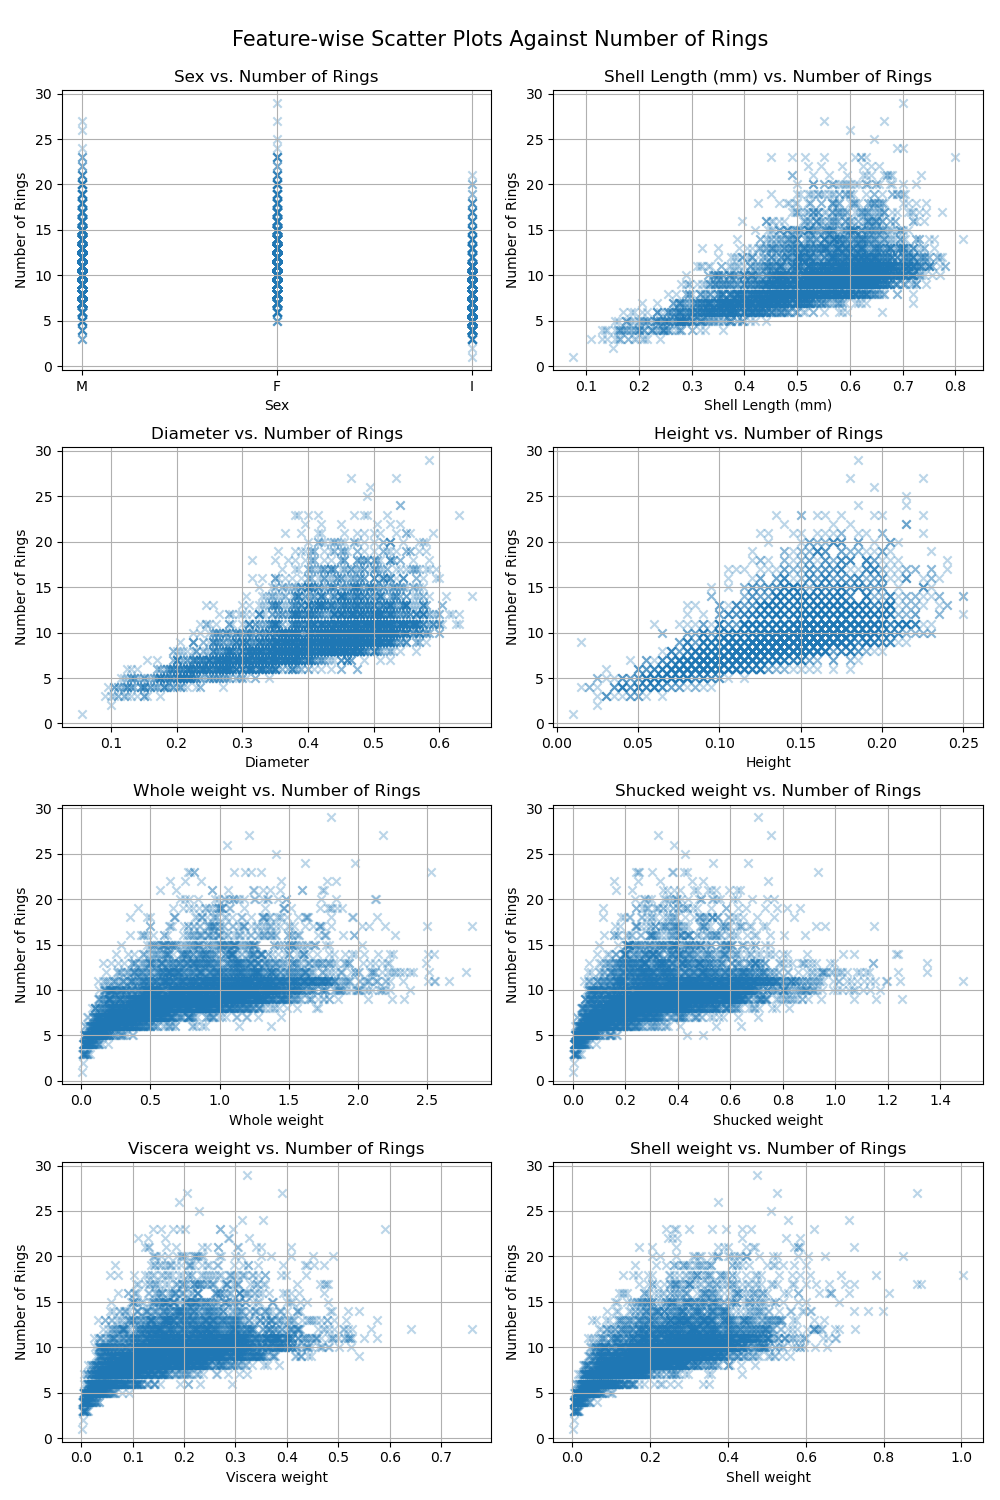
\includegraphics[width=0.8\textwidth]{Figures/Feature_wise_Scatter_Plots_Against_Number_of_Rings.png}
    \caption{Scatterplots visualizing the relationship between individual features and the number of turtles in the dataset after data cleaning.}
    \label{fig:all_features_datasets}
\end{figure}

\begin{figure}[h]
    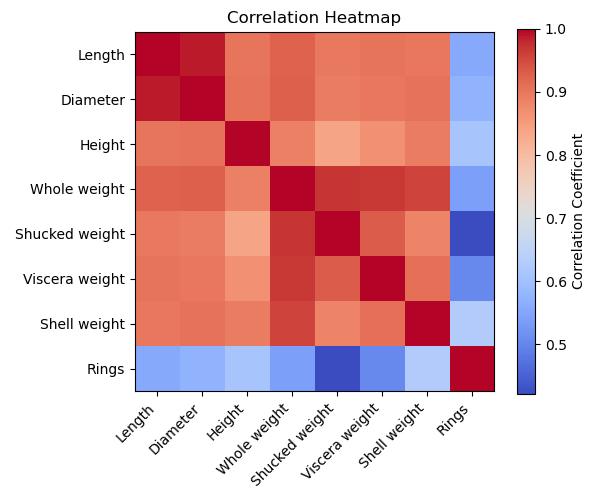
\includegraphics[width=\linewidth]{Figures/Correlation_Heatmap.png}
    \caption{Heatmap visualizing the correlation matrix between all numerical features.}
    \label{fig:heatmap}
\end{figure}

\begin{figure}[h]
    \centering
    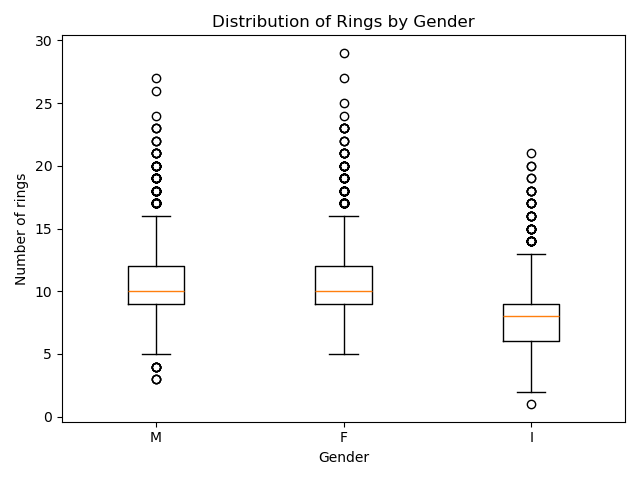
\includegraphics[width=\textwidth]{Figures/Distribution_of_Rings_by_Gender.png}
    \caption{Boxplots visualizing the distribution of number of rings for each gender individually.}
    \label{fig:gender_boxplots}
\end{figure}

\begin{figure}[h]
    \centering
    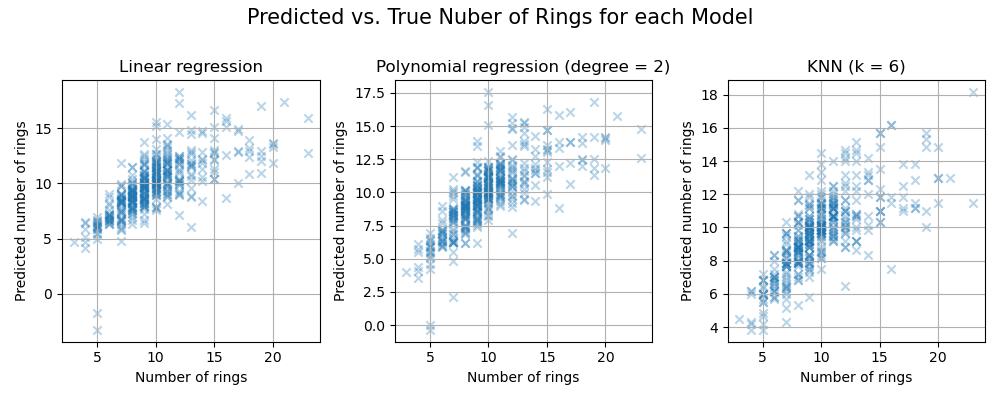
\includegraphics[width=\textwidth]{Figures/Predicted_vs._True_Nuber_of_Rings_for_each_Model.png}
    \caption{Scatterplots comparing the test set predictions with the true number of rings separately for each model.}
    \label{fig:model_predictions}
\end{figure}

\begin{figure}[h]
    \centering
    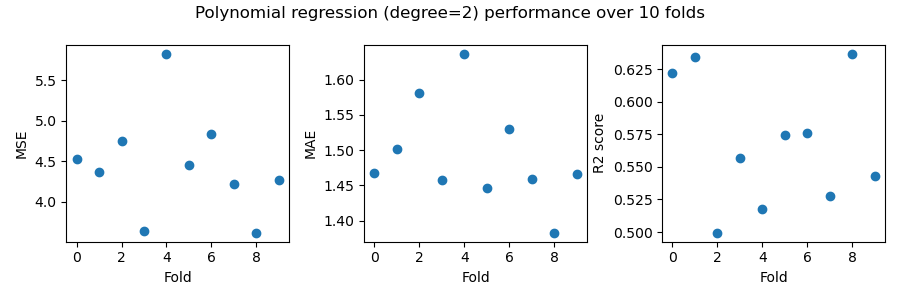
\includegraphics[width=\textwidth]{Figures/Polynomial_regression__degree_2__performance_over_10_folds.png}
    \caption{Scatterplots displaying different evaluation metrics for the predictions of the 2nd-degree polynomial model over 10 folds.}
    \label{fig:polynomial_fold_valuation}
\end{figure}

\begin{figure}[h]
    \centering
    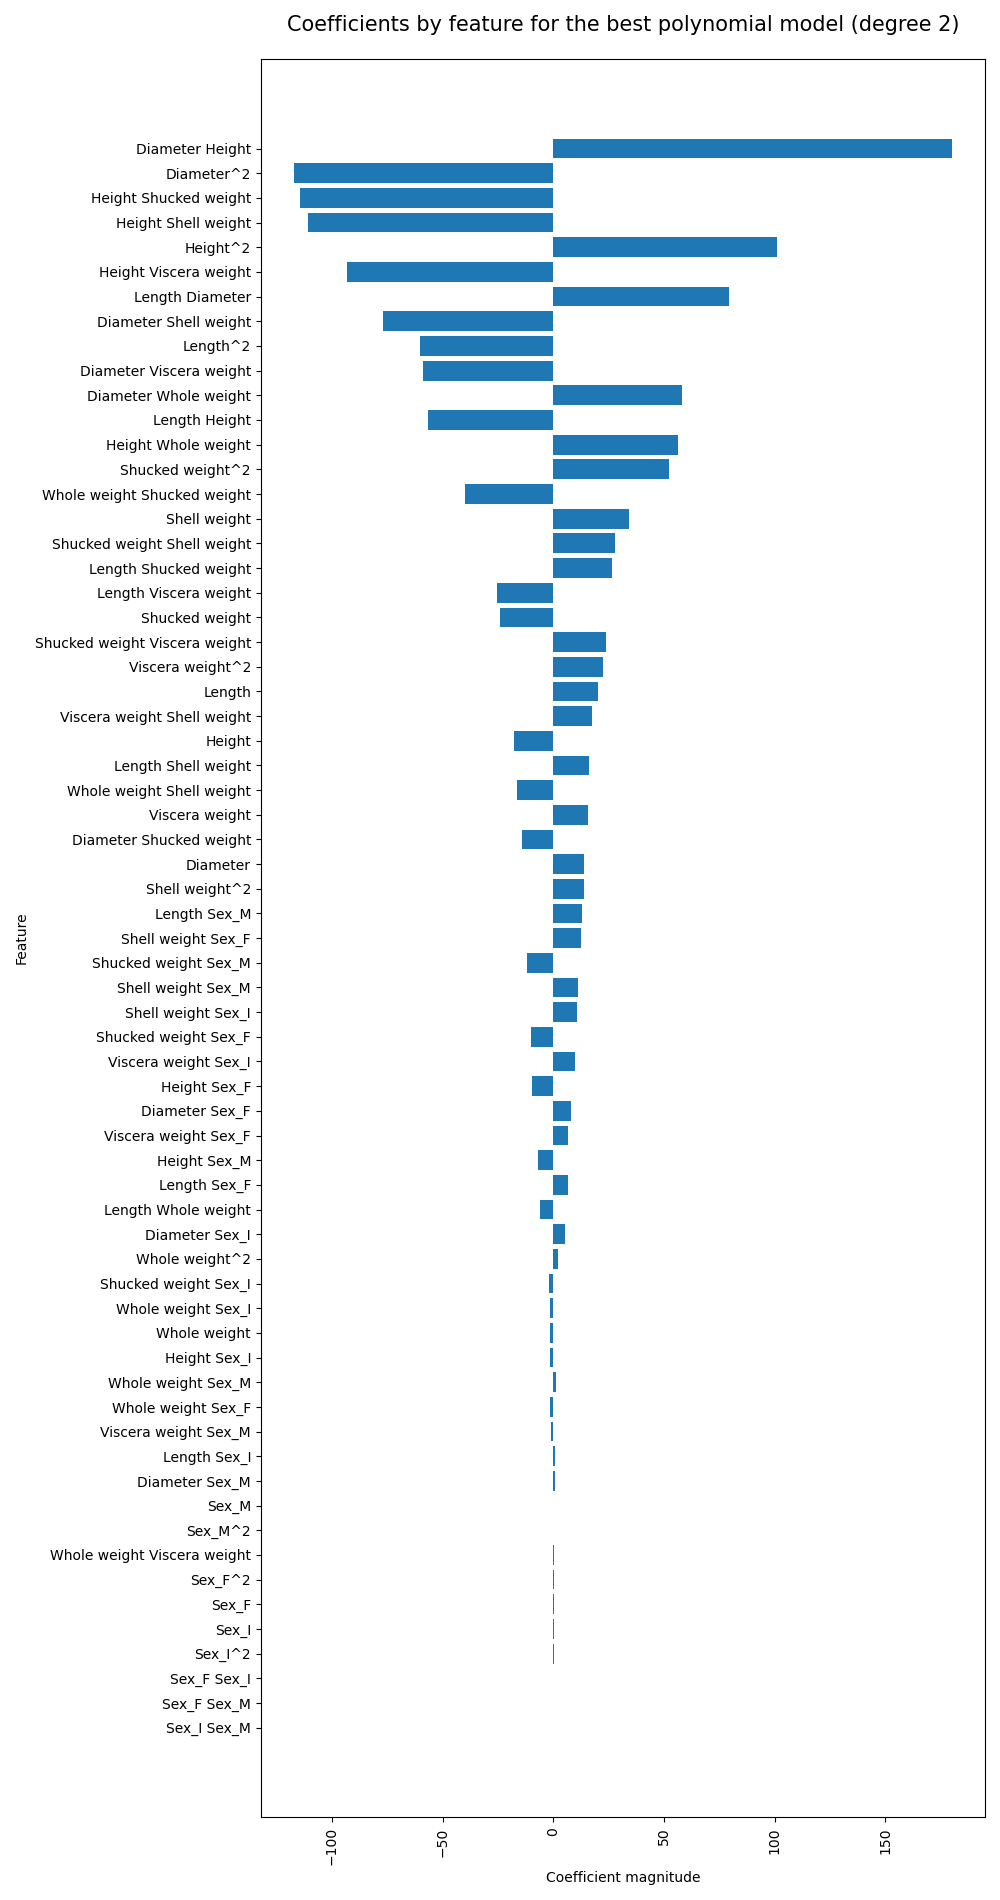
\includegraphics[width=0.65\textwidth]{Figures/Coefficients_by_feature_for_the_best_polynomial_model__degree_2_.png}
    \caption{Bargraph displaying the magnitude of coefficients for each feature in the 2nd degree polynomial model on its best run during the 10-fold-cross-validation. Features were sorted by coefficient magnitude.}
    \label{fig:coefficient_magnitudes}
\end{figure}

\begin{figure}[h]
    \centering
    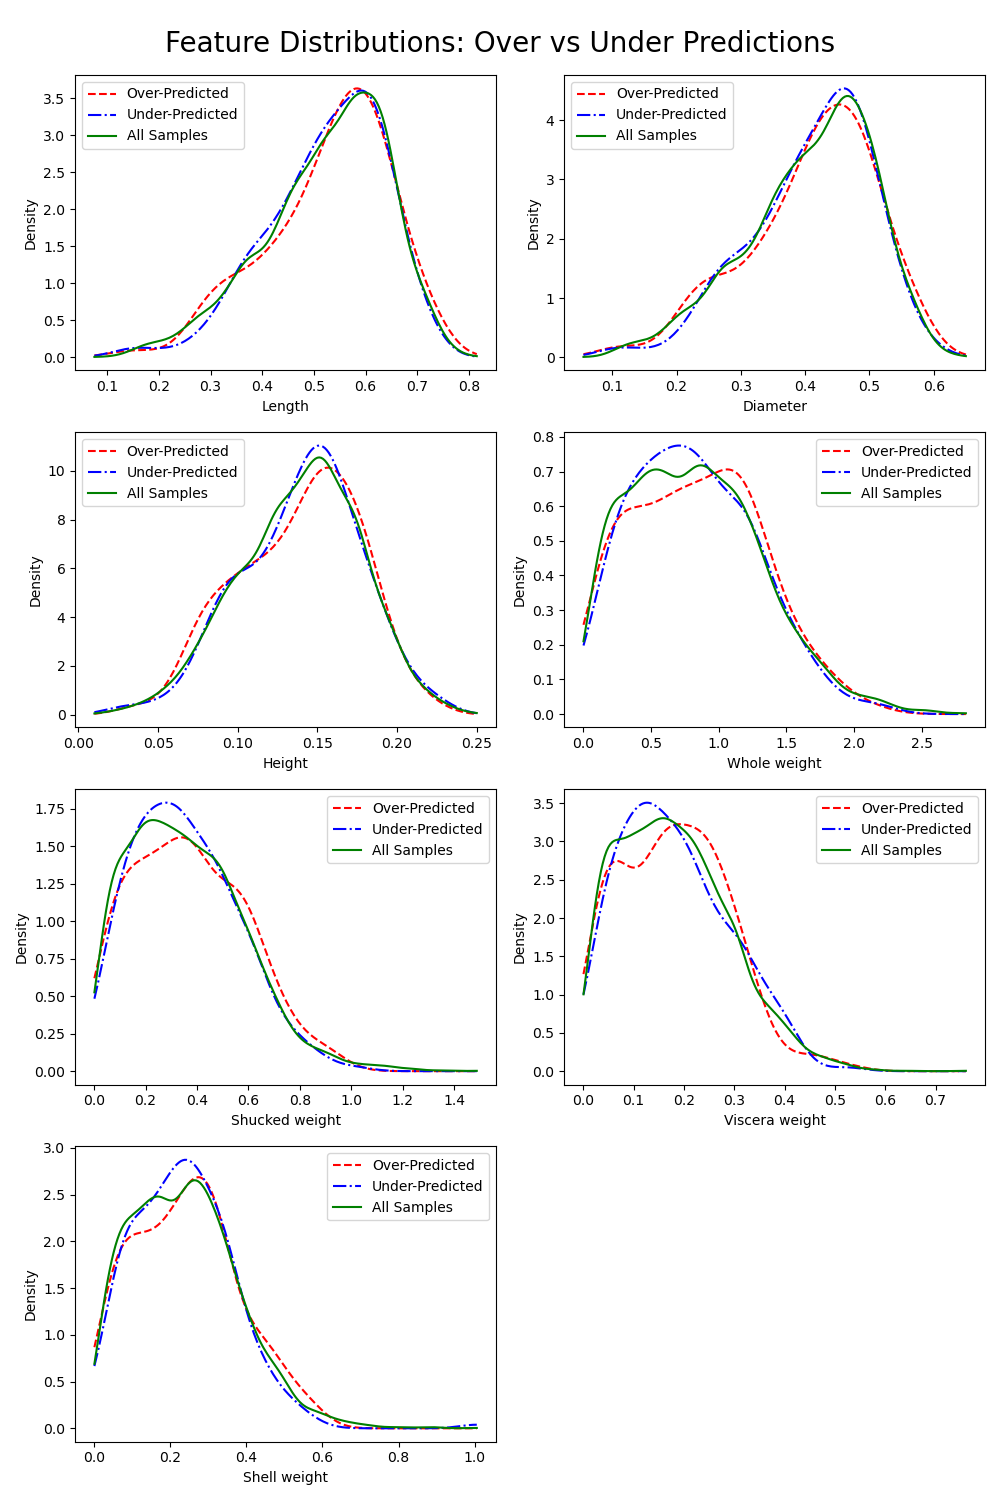
\includegraphics[width=0.85\textwidth]{Figures/Feature_Distributions__Over_vs_Under_Predictions.png}
    \caption{Kernel density estimates for each numerical feature comparing over-predicted, under-predicted, and all samples.}
    \label{fig:over_underprediction_density}
\end{figure}

\begin{figure}[h]
    \centering
    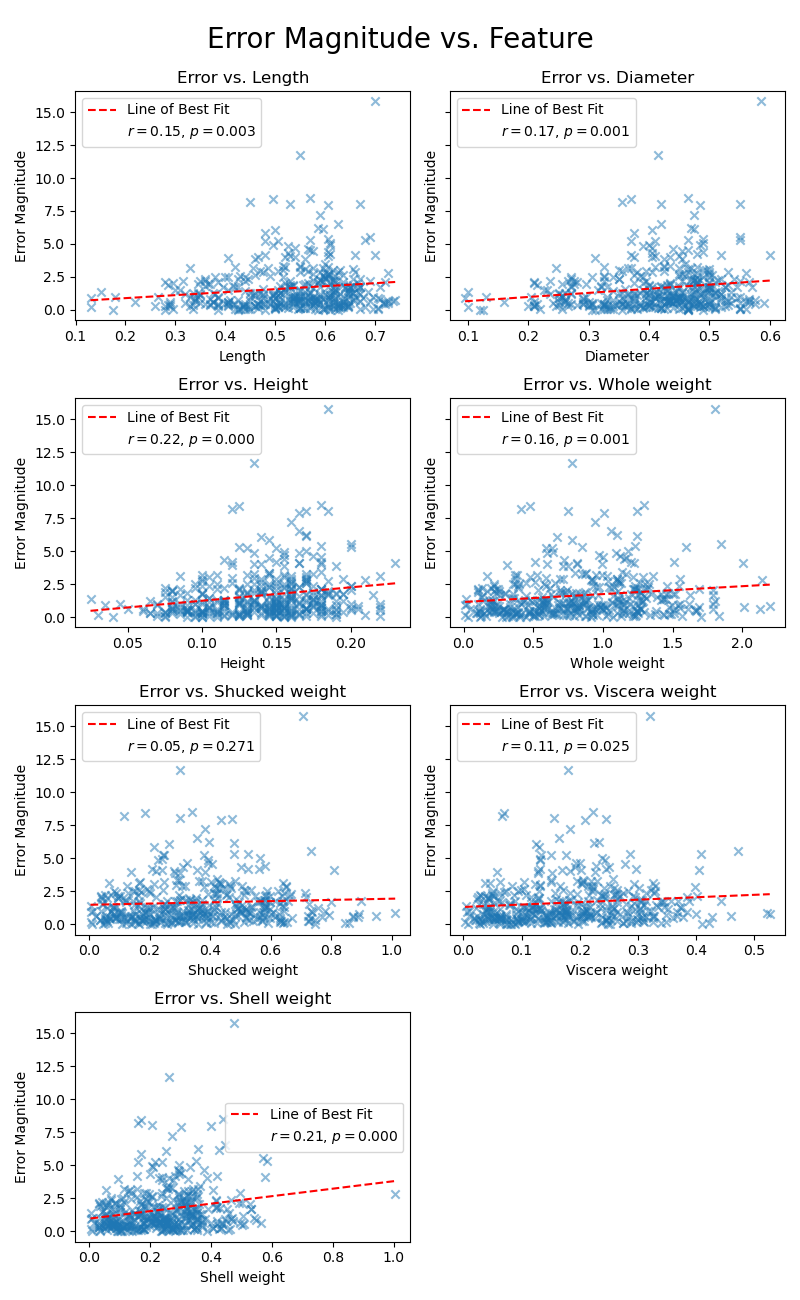
\includegraphics[width=0.75\textwidth]{Figures/Error_Magnitude_vs._Feature.png}
    \caption{Scatter plots visualizing the error magnitude in relation to the values of individual features in the dataset. The values are retrieved from the worst run of the 10-fold cross-validation of the 2nd-degree polynomial regressor.}
    \label{fig:error_magnitude_by_feature}
\end{figure}

\end{document}